\documentclass{article}
% set margins
\usepackage[left=1.5in, right=1in, top=1in, bottom=1in]{geometry}
% add spacing
\usepackage{setspace}
% use biblatex
\usepackage[style=numeric]{biblatex}
% add the bibliography
\addbibresource{bibliography.bib}
% remove dots in TOC
\usepackage[titles]{tocloft}
\renewcommand{\cftdot}{}

\usepackage{amssymb}
\usepackage{amsmath}

% unbold things
\usepackage{titlesec}
\titleformat*{\section} {\centering} % format
\titleformat*{\subsection}{\centering \normalfont}
\titleformat*{\subsubsection}{\normalfont}

% format the table of contents
\usepackage[]{tocstyle}
\usetocstyle{standard}
\makeatletter
\renewcommand\tableofcontents{
  \null\hfill\MakeUppercase{\contentsname}\hfill\null\par
  \hfill \break
  \@starttoc{toc}}
\makeatother
\setcounter{tocdepth}{2}

% use images from the 'images' directory
\usepackage{graphicx}
\graphicspath{{images/}}

% metadata
\title{Exploring Semantic Hierarchies to Improve Resolution Theorem Proving on Ontologies}
\author{Stanley C. Small}
\date{March 2019}

\begin{document}
\begin{titlepage}
	\makeatletter
		\begin{center}
   				\MakeUppercase{\@title} \par
  				\smallskip 
 				\vspace{.15in} by \par
 				\smallskip
  				\vspace{.15in} \@author \par
  				\vspace{1in}
 				A Thesis Submitted in Partial Fulfillment  \par
  				of the Requirements for a Degree with Honors \par
  				(Computer Science) \par
  				\vspace{.75in}
  				The Honors College \par
  				University of Maine \par
  				\@date \par
 				\vfill
   		\end{center}
	\makeatother
	\begin{flushleft}
		Advisory Committee: \\
		\hspace{.3in} Dr. Torsten Hahmann, Assistant Professor$^{1}$, Advisor \\
		\hspace{.3in} Dr. Mark Brewer, Professor of Political Science \\
		\hspace{.3in} Dr. Max Egenhofer, Professor$^{1}$ \\
		\hspace{.3in} Dr. Sepideh Ghanavati, Assistant Professor$^{1}$ \\
		\hspace{.3in} Dr. Roy Turner, Associate Professor$^{1}$ \\
		\hfill \break
		\hspace{.3in} $^{1}$School of Computing and Information Science
	\end{flushleft}
\end{titlepage}

\pagenumbering{gobble}
\newpage
\addcontentsline{toc}{section}{\MakeUppercase{Abstract}}
\setstretch{2}
\vspace*{.05in}
\section*{\MakeUppercase{Abstract}}
A resolution-theorem-prover (RTP) evaluates the validity (truthfulness) of conjectures against a set of axioms in a knowledge-base. When given a conjecture, an RTP attempts to resolve the negated conjecture with axioms from the knowledge-base until the prover finds a contradiction. If the RTP finds a contradiction between the axioms and a negated conjecture, it proves the conjecture. 

The order in which the axioms within the knowledge-base are evaluated significantly impacts the runtime of the program, as the search-space increases exponentially with the number of axioms. 

Ontologies, knowledge bases with semantic (and predominantly hierarchical) structures, describe objects and their relationships to other objects. For example, a 'Car' class might exist in a sample ontology with 'Vehicle' as a parent class and 'Bus' as a sibling class. Currently, any hierarchical structures within an ontology are not taken into account when evaluating the relevance of each axiom. At present, each predicate is automatically assigned a weight based on a heuristic measure (such as the number of terms or the frequency of predicates relevant to the conjecture) and axioms with higher weights are evaluated first. My research aims to intelligently select relevant axioms within a knowledge-base given a structured relationship between predicates. I will use the semantic hierarchy over predicates to assign weights to each predicate passed to a weighting function. The research aims to design heuristics based upon the semantics of the predicates, rather than solely the syntax of the statements. 

I plan to develop weighting functions based upon various parameters relevant to the ontological structure of predicates contained in the ontology, such as the size and depth of a hierarchy based upon the structure of the ontology. 

I will implement methods to calculate weights for each predicate and thus each axiom in attempts to select relevant axioms when proving a theorem. Then, I will conduct an experimental study to determine if my methods show any improvements over current reasoning methods.
	
\pagenumbering{roman} 
\setcounter{page}{3}
\newpage
\addcontentsline{toc}{section}{\MakeUppercase{Acknowledgements}}
\vspace*{.05in}
\section*{\MakeUppercase{Acknowledgements}}
        
Many thanks are given to Dr. Hahmann. This work could not be completed without his continued support and encouragement. Despite his tremendously busy schedule, he always made time to meet and answer questions. 

Robert Powell also proved instrumental to the process. His utility which converts Common Logic Interchange Format (CLIF) into web ontology language (OWL). His work streamlined the testing process and allowed me to find necessary results. 

The thesis committee was also instrumental in producing this undergraduate thesis.

\newpage
\addcontentsline{toc}{section}{\MakeUppercase{List of Figures}}
\vspace*{.05in}
\listoffigures

\newpage
\addcontentsline{toc}{section}{\MakeUppercase{List of Tables}}
\vspace*{.05in}
\listoftables

\newpage
\setstretch{1.5}
\tableofcontents

\newpage
\setstretch{2}
\pagenumbering{arabic}
\setcounter{page}{1}
\vspace*{.05in}
\section{\MakeUppercase{Introduction}}

The rules of logic enable one to prove theorems from axioms stored in a knowledge-base. Axioms, asserted facts typically expressed in a formal manner, provide a computer program with tools to confirm or refute conjectures without additional user input. Because computers excel at simple and repetitive tasks, one can witness the applications of automated theorem proving in fields which rely heavily on "knowledge acquisition and information retrieval" \cite{sanchez2012ontology}. The ability for machines to deduce logically valid conclusions has applications in artificial intelligence and a variety of scientific domains. Automated theorem proving provides a versatile method for reasoning with a set of facts, and has been used to prove and verify proofs of multiple theorems. The four color map theorem, obtained by an automated proof in 1976 by a general-purpose theorem-proving software in 2005 remains a notable example \cite{gonthier2008formal}. Moreover, advances have been made in work on the Kepler conjecture and in finding optimal solutions for a Rubik's Cube. The general-purpose nature of automated theorem proving yields applications to a variety of problems. However, automated theorem proving programs often neglect semantic knowledge embedded in an ontology.

Ontologies provide a "common vocabulary" for researchers to speak about a specific domain by describing entities and the relationships between them \cite{noy2001ontology}. A formal description of a specific environment provides researchers and machines with a shared understanding by aiming to capture the semantics of a domain's concepts and relations. Some relationships between an ontology's terms may be explicitly defined, but many are implicit. 

\begin{singlespace}
\[isSedan(Subaru Legacy)\]
\[\forall x \; isSedan(x) \rightarrow isAutomobile(x)\]
\end{singlespace}

The former axiom asserts a Subaru Legacy is a sedan and the latter asserts all sedans are automobiles. While one can easily deduce the fact a Subaru Legacy is an automobile, no single axiom explicitly describes such a statement. Fortunately, formal logic defines rules of inference which allow one to transform established facts into new conclusions solely based on the syntax of these statements. Both humans and computers can clearly distinguish well formed statements ($x+y=4$) from those which are not ($x4y+=$). Beyond the syntax of statements, ontologies and logics also define the semantics or meaning of sentences (i.e. declaring $x+y=4$ is true when $x=1$ and $y=3$ but false when $x=0$ and $y=1$). 

Like many taxonomies, one can often form maps of relationships within an ontology which resemble a hierarchy. Currently, knowledge encoded in semantic hierarchies constructed from ontologies is not taken into account when determining which axioms might be most helpful when attempting to prove a specific theorem. This work attempts to improve automated theorem proving with ontologies by identifying relevant facts, and ignoring those less likely to yield a proof.

%Try to use some very simple examples, e.g., a toy ontology, specific domains for ontologies, the kind of relations we can find therein (subclass and subproperty, domain and range restrictions), what the semantic hierarchy looks in the example, an example how the semantic hierarchy may help in a proof (when there are lots of irrelevant axioms).

DESCRIPTION OF THE CONCRETE OBJECTIVE AND APPROACH OF YOUR WORK

\newpage
\vspace*{.05in}
\section{\MakeUppercase{Background and Related Work}}
\subsection{{Ontologies}}

 The word ontology ("study of being") combines Greek \textit{onto-} ("being") and \textit{-logia} ("logical discourse"). The act of studying knowledge and existence in philosophy has given birth to the study of formal logic and automated reasoning in computer science. Researchers often use ontologies to share information among people or computer programs, to enable domain knowledge reuse, to make definitions of a particular domain explicit, or to analyze domain knowledge \cite{noy2001ontology}. While ontologies can often witness reuse, ontology design rarely encounters a single best solution satisfying all goals of the ontology. 
 
\begin{figure}[h]
\centering
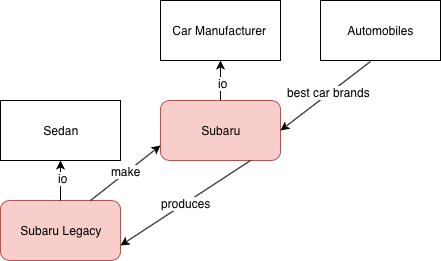
\includegraphics[width=4in]{sample_ontology}
\caption{This simple ontology describes classes (black) and instances (red) in the "automobiles" ontology (inspiration from an example by Natalya F. Noy) \cite{noy2001ontology}.}
\label{fig:sample_ontology}
\end{figure}

 
In reality, few differences between an ontology and a knowledge base exists. Knowledge engineers must traverse a "fine line where the ontology ends and the knowledge base begins" \cite{noy2001ontology}. At the least, an ontology defines categories (or classes) and relationships among objects.One can think of an ontology as a "vocabulary" used to describe a domain \cite[308]{russell2016artificial}. Typically, the classes can be arranged in a hierarchy and the relationships into a separate hierarchy, which are here referred to as semantic hierarchies. When designing an ontology, one must decide the scope and organization of the knowledge, along with the language used to describe a specific domain. Refer to Figure \ref{fig:sample_ontology} for an example. 


% Explain the terms and they structure knowledge and how inheritance works

At a simplistic level, semantic hierarchies describing an ontology can be compared to a family tree. Given a pair of two individuals, if one were tasking with determining if two individuals are related, a family tree would prove quite useful. 

First order logic exists as one possible language to describe ontologies. 

\subsection{{Theorem Proving}}
Formal logics like first-order logic defines a structure for statements which can be used to form logical and mathematical proofs. Asserted facts, called axioms, are used to derive facts which logically follow. Consider the following set of facts. 

\begin{singlespace}
\[isSedan(Subaru Legacy)\]
\[\forall x \; isSedan(x) \rightarrow hasFourSeats(x)\]
\end{singlespace} 

The first statement asserts the Subaru Legacy is a sedan. The second statement asserts all sedans have four seats. These two statements do not directly state the Subaru Legacy has four seats. However, one can derive the statement $hasFourSeats(Subaru Legacy)$ by using the inference rule \textit{modus ponens}, defined below. 
\begin{singlespace}
\[A\]
\[A \rightarrow B\]
 \[\therefore B\]
\end{singlespace} 

One can think of $A$ and $B$ as variables representing statements, and any statement can replace them. An inference rule defines a valid rule for statements. By expressing facts in a formal notation, one makes proofs using such statements mechanical and easily parsed by a computer. Expressing statements in formal logic poses multiple challenges. First, each object and relationship must be explicitly defined.

Resolution is one of many methods for automated theorem proving. Historically, resolution has significance and is widely used \cite[51]{ertel2018introduction}.
In order to use resolution as a proof technique, axioms must first be expressed in Conjunctive Normal Form. This can be done by follwing a 7-step procedure of converting the set of facts into a conjunction of disjunctions. 
\begin{singlespace}
 \[isSedan(X) \rightarrow hasFourSeats(X)\]
\[\lnot isSedan(X) \lor hasFourSeats(X)\]
One can then resolve the statements. 
\[\frac{isSedan(Subaru Legacy), \lnot isSedan(X) \lor hasFourSeats(X)}{hasFourSeats(Subaru Legacy)}\]
\end{singlespace} 

\begin{figure}[h]
\centering
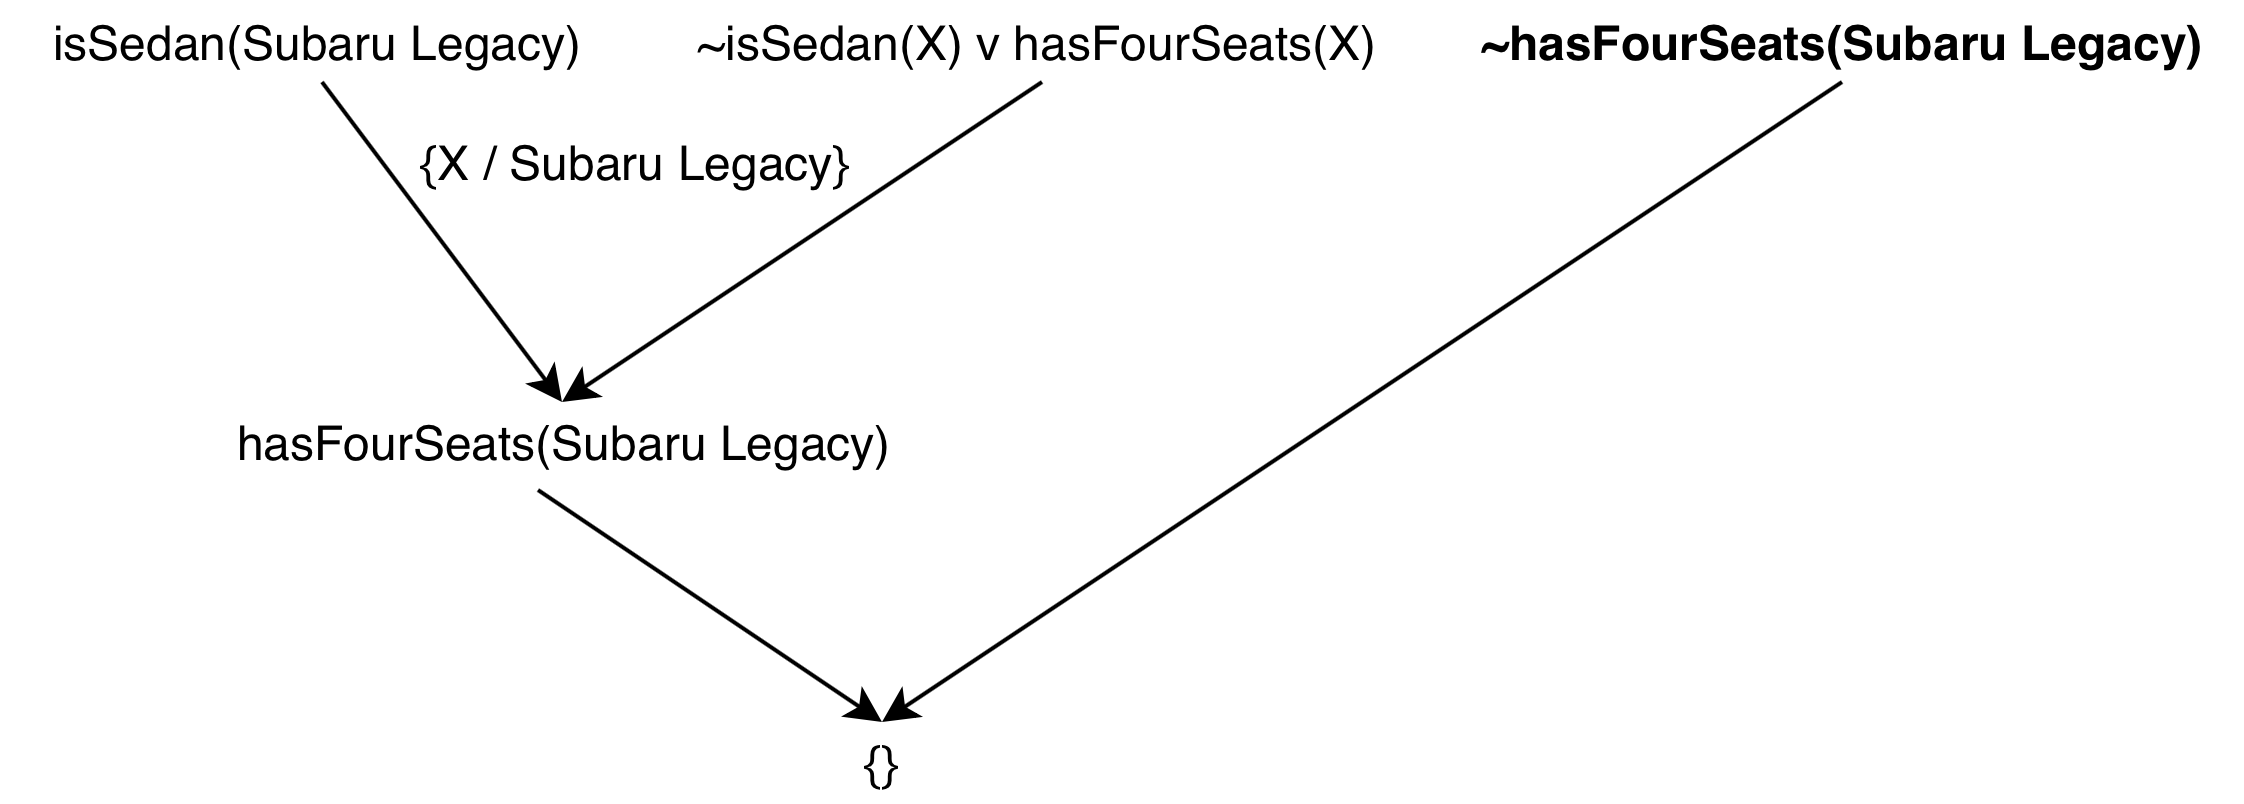
\includegraphics[width=6in]{resolution_tree}
\caption{This shows a resolution tree.}
\label{fig:resolution_tree}
\end{figure}

\begin{figure}[h]
\centering
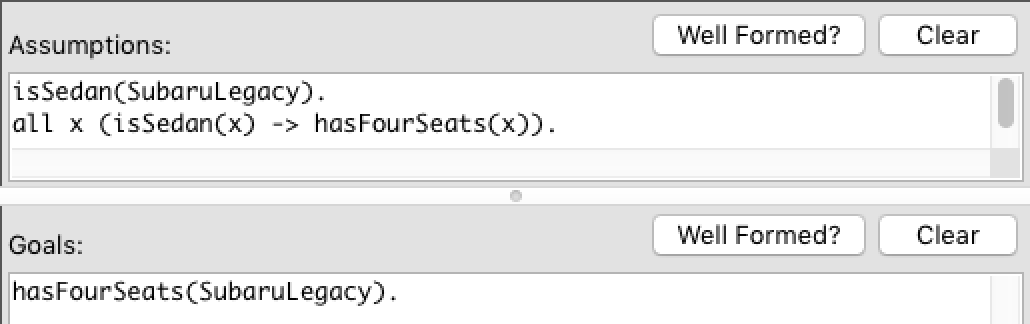
\includegraphics[width=6in]{prover9input}
\caption{This shows the input into the prover9 program}
\label{fig:prover9input}
\end{figure}

\begin{figure}[h]
\begin{verbatim}
1 (all x (isSedan(x) -> hasFourSeats(x))) # label(non_clause).  [assumption].
2 hasFourSeats(SubaruLegacy) # label(non_clause) # label(goal).  [goal].
3 -isSedan(x) | hasFourSeats(x).  [clausify(1)].
4 isSedan(SubaruLegacy).  [assumption].
5 hasFourSeats(SubaruLegacy).  [resolve(3,a,4,a)].
6 -hasFourSeats(SubaruLegacy).  [deny(2)].
7 $F.  [resolve(5,a,6,a)].
\end{verbatim}
\caption{This shows the Prover9 output for the above proof.}
\label{fig:prover9out}
\end{figure}

In resolution, the search space increases exponentially with the addition of each new axiom.

\subsection{{Semantic Similarity}}
One straightforward method of calculating the semantic similarity between two entities in an ontology. 

In an undirected graph $G$ defined as a pair $(V,E)$, where $V$ is a set of vertices, and $E$ is a set of edges between the vertices $E \subseteq {(u,v) | u, v \in V}$, one can define a path $path(a,b)=l_{1,\dots ,}l_k$ as a set of links connecting $a$ and $b$ in a taxonomy and $\lvert path(a,b) \rvert = k$ as the length of the path \cite{sanchez2012ontology}. One can calculate the semantic distance between $a$ and $b$ using equation \ref{rada} \cite{rada1989development}.

\begin{equation}
sim(a,b)=min_{\forall i}\lvert{path_i(a,b)}\rvert
\label{rada}
\end{equation}
By incorporating depth of the taxonomy into the function, improvement has been seen \cite{wu1994verbs}.
\begin{equation}
sim(a,b)=\frac{2 \times N_3}{N_1+N_2+2 \times N_3}
\label{wu}
\end{equation}

\newpage
\vspace*{.05in}
\section{\MakeUppercase{Approach}}
In efforts to quantitatively evaluate the effectiveness of the proposed weighting functions, a series of experiments were conducted on multiple ontologies. The ontologies selected for testing exist in the COmmon Logic Ontology REpository (COLORE). The objective of COLORE is to serve as a "testbed for ontology evaluation and integration techniques" \cite{gruninger2012specifying}. Code from the project can be found at \url{https://code.google.com/p/colore}. 

My experiments were conducted using Prover9, written by William McCune \cite{mccune2005prover9}. Many tests were conducted using a version of the program which supports a GUI, but a command line version is available for running automated tests. 
Git was used for version control and a repository containing source code can be found at \url{https://github.com/stanleysmall/thesis}.

\begin{figure}[h]
\centering
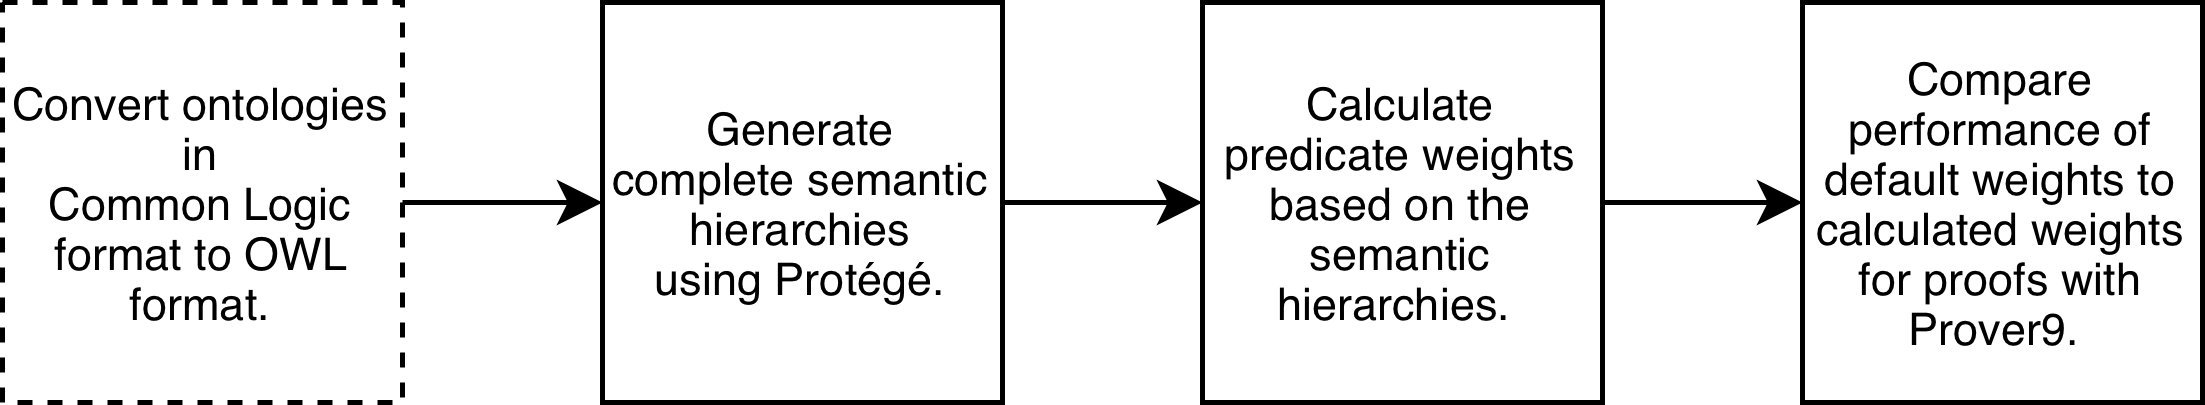
\includegraphics[width=6in]{flowchart}
\caption{An illustration of my process.}
\label{fig:flowchart}
\end{figure}

\subsection{Converting Ontologies}
COLORE 


\subsection{Generating a Complete Heirarchy}

Given an ontology and a conjecture, one can generate weights for classes and properties to reduce the number of clauses generated in a proof. Functions are evaluated by their influence on the number of clauses generated with a proof. 

After a hierarchy has been generated, weights can be assigned to each class and subproperty. The same weighting function is applied to both the classes and sub-properties. 

The weighting functions are currently applied by hand to the ontologies, with the beginnings of an automated program underway. 



\subsection{{Default Weights}}
\begin{figure}[h]
\centering
\begin{itemize}
    \item The default weight of a constant or variable is 1.
    \item The default weight of a term or atomic formula is one more than the sum of the weights of its arguments.
    \item The default weight of a literal is the weight of its atomic formula.
    \item The default weight of a clause is the sum of the weights of its literals.
\end{itemize}
\caption{These are the default weights in the Prover9 program \cite{mccune2005prover9}.}
\label{fig:default_weights}
\end{figure}

\begin{figure}[h]
\centering
\begin{verbatim}
list(weights).
  weight(a)=3.                         % the weight of the constant a is 3
  weight(f(a,x))=5*weight(x).          % weight(f(a,term))=5*weight(term)
  weight(f(a,_))=-1.                   % _ matches any variable
  weight(x|y)=2+(weight(x)+weight(y)). % add 2 for each "or" symbol
end_of_list.
\end{verbatim}
\caption{These are example weights given to the Prover9 program \cite{mccune2005prover9}.}
\label{fig:example_weights}
\end{figure}

\subsection{Computing Weighting Functions}

\newpage
\vspace*{.05in}
\section{\MakeUppercase{Experiments}}

\subsection{{Setup}}


\begin{figure}[h]
\centering
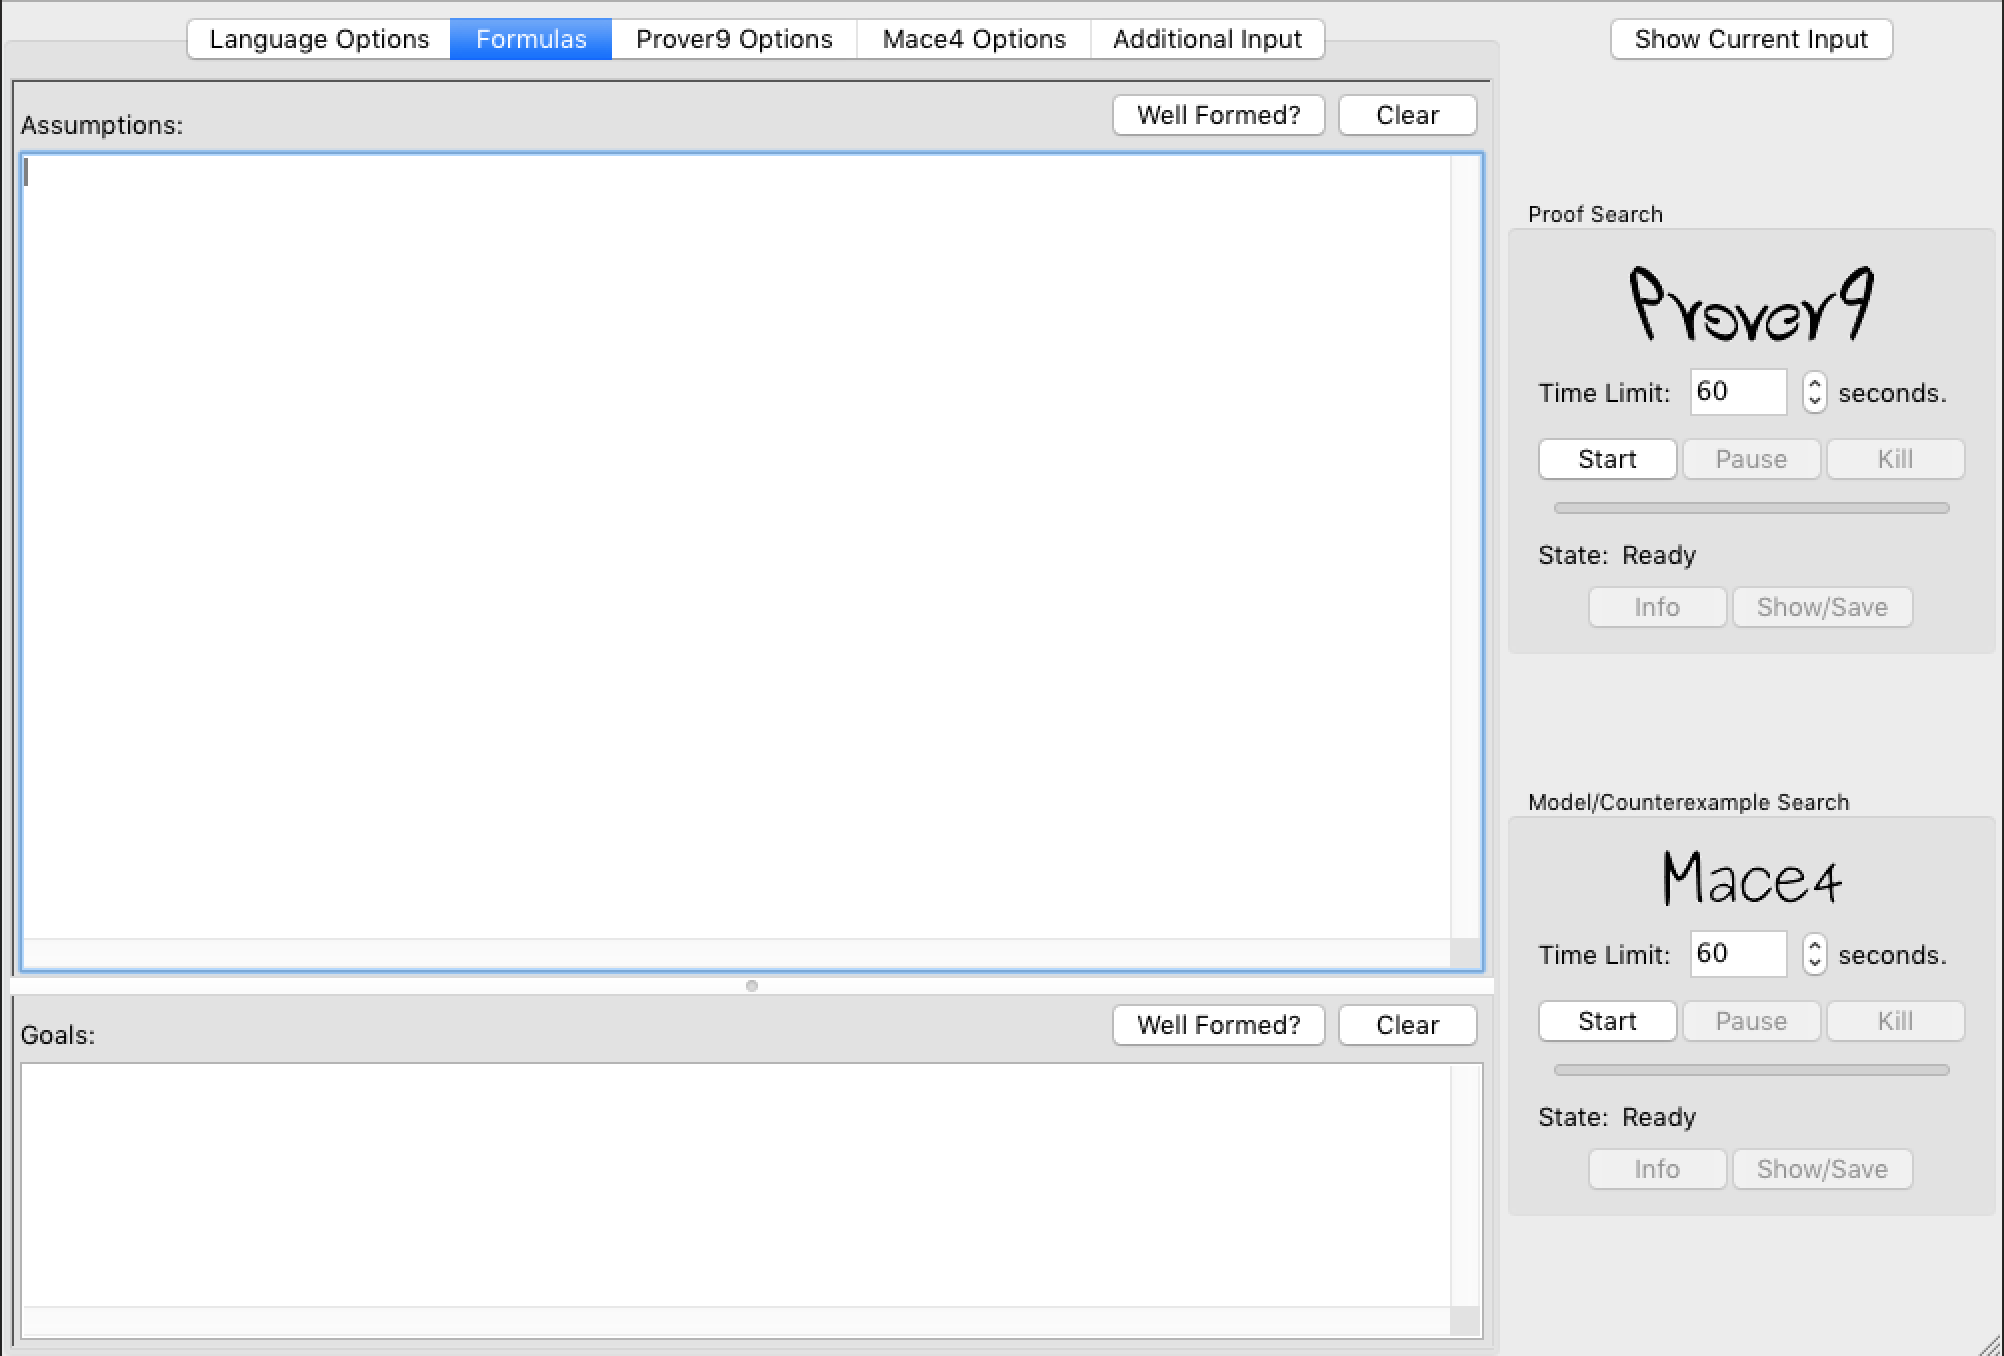
\includegraphics[width=6in]{prover9}
\caption{The graphical user interface for Prover9 on macOS \cite{mccune2005prover9}.}
\label{fig:prover9}
\end{figure}



\subsection{{Results}}
\subsubsection{multidim\_space\_voids}



\newpage
\vspace*{.05in}
\section{\MakeUppercase{Conclusions}}

In many cases, the algorithm increases the number of clauses generated for each test, but does not do so to the point where the tests are unusable. For some very specific ontologies, the number of clauses generated decreases. This can be attributed to, in part, by the small number of ontologies available for testing, along with the specific pattern and hierarchy of each ontology. 

Many opportunities for further research include fully automating the search procedure, working with a larger number of ontologies to ensure the weighting functions actually do as they say, developing a new approach towards automatically weighting the predicates. 
\newpage
\addcontentsline{toc}{section}{\MakeUppercase{References}}
\vspace*{.05in}
\printbibliography

\newpage
\appendix

\section{\MakeUppercase{Tests}}

\newpage
\addcontentsline{toc}{section}{\MakeUppercase{Author's Biography}}
\vspace*{.05in}
\section*{\MakeUppercase{Author's Biography}}
Stanley C. Small grew up in Hampden, Maine with his mother Diane and his father Scott. He attended the University of Maine and received a Bachelor of Science degree in Computer Science in May of 2019. 


\end{document}
